\documentclass[12pt,aspectratio=169]{beamer}

\usetheme[progressbar=frametitle]{metropolis}
\usepackage{appendixnumberbeamer}
\usepackage{booktabs}
\usepackage[scale=2]{ccicons}
\usepackage{listings}
\usepackage{spot}
\usepackage{pgfplots}
\usepgfplotslibrary{dateplot}

\usepackage{xspace}
	%\definecolor{almond}{rgb}{0.94, 0.87, 0.8}
		\definecolor{cornsilk}{rgb}{1.0, 0.97, 0.86}
%\definecolor{Purple}{HTML}{911146}
%	\definecolor{coolblack}{rgb}{0.0, 0.18, 0.39}
%\setbeamercolor{frametitle}{bg=coolblack}
	%\definecolor{burgundy}{rgb}{0.5, 0.0, 0.13}
	%\definecolor{bluep}{rgb}{0.2, 0.2, 0.6}
		\definecolor{darkslateblue}{rgb}{0.28, 0.24, 0.55}
%\definecolor{vsplblue}{HTML}{00a1e5}
%\setbeamercolor*{palette primary}{fg=vsplblue!60!black,bg=gray!30!white}
%\setbeamercolor{titlelike}{fg=darkslateblue}
\setbeamercolor{frametitle}{fg=prussianblue,bg=white}
%\definecolor{vsplbggray}{HTML}{efefef}
\definecolor{ivory}{rgb}{1.0, 1.0, 0.94}
	\definecolor{junglegreen}{rgb}{0.16, 0.67, 0.53}
		\definecolor{persiangreen}{rgb}{0.0, 0.65, 0.58}
\setbeamercolor{progress bar}{fg=persiangreen}
\setbeamercolor{alerted text}{fg=persiangreen}
%\definecolor{myteal}{HTML}{44AA99}
	%\definecolor{darkslateblue}{rgb}{0.28, 0.24, 0.55}
%\definecolor{myred}{HTML}{661100}
%\setbeamercolor{background canvas}{bg=red}
	\definecolor{prussianblue}{rgb}{0.0, 0.19, 0.33}
	\definecolor{gray}{rgb}{0.5, 0.5, 0.5}
%% This is pretty good; tan, seagreen, dark blue
	%	\definecolor{darkslateblue}{rgb}{0.28, 0.24, 0.55}
%\definecolor{ivory}{rgb}{1.0, 1.0, 0.94}
	%\definecolor{junglegreen}{rgb}{0.16, 0.67, 0.53}
	%	\definecolor{persiangreen}{rgb}{0.0, 0.65, 0.58}
		\definecolor{slategray}{rgb}{0.44, 0.5, 0.56}
%\setbeamercolor{progress bar}{fg=persiangreen}
%\setbeamercolor{titlelike}{fg=darkslateblue}
%\setbeamercolor{frametitle}{fg=darkslateblue,bg=ivory}


\setbeamercolor{titlelike}{fg=white}
%\setsansfont[BoldFont={Fira Sans SemiBold}]{Fira Sans Book}

\title{Bootstrapping Confidence Intervals \\ (with Confidence!)}
%\subtitle{A modern beamer theme}
% \date{\today}
\date{}
\author{Aaron Kaufman}
\institute{November 16, 2018}
	

\begin{document}

{\setbeamercolor{background canvas}{bg=prussianblue}
\setbeamercolor{normal text}{fg=white}
\maketitle
}

\setbeamercolor{normal text}{fg=gray}\usebeamercolor*{normal text}

\begin{frame}
\frametitle{Previously: Calculating Confidence Intervals}

\uncover<2->{\textbf{Statistics:} science of uncertainty, \uncover<3->{and CIs are our most important tool}}


\uncover<4->{\textbf{95\% Confidence Interval:} \uncover<5->{ If we construct 100 such intervals, 95\% will contain the truth}}

\uncover<6->{\textbf{Procedure:}}
\begin{enumerate}
	\item<7->{Collect a sample of data from the population}
	\item<8->{Calculate a quantity of interest, \textbf{X}}
	\item<9->{Calculate a standard deviation, \textbf{$s$}}
	\item<10->{Calculate a standard \textbf{error} \textbf{$\sigma$}: $\frac{s}{\sqrt{n}}$} 
	\item<11->{Use a Z-table to figure out how many SEs you need \uncover<12->{(1.96 for 95\%, 2.58 for 99\%)}}
	\item<13->{For 95\%: $[X - 1.96 \times \sigma, X + 1.96 \times \sigma]$}
\end{enumerate}

\end{frame}

%% We know how to calculate a confidence interval using the normal distribution, and what they're used for. 
%% We find the standard deviation of our estimate, maybe an average, calculate the standard deviation, and if we want a 95\% confidence interval, multiply by about 1.96, then our confidence intervial is our average +/- 1.96 * SD. 

\begin{frame}
\frametitle{Previously: Calculating Confidence Intervals}

\uncover<2->{\textbf{Data:} \uncover<3->{2016 American National Election Study (4,142 US adults)}}

\uncover<2->{\textbf{Example:} \uncover<4->{What percentage of adult US residents are registered to vote?}}


\begin{enumerate}
	\item<5->{\textbf{Average:} 85.7\%}
	\item<6->{\textbf{Standard Deviation:} 35.0\%}
	\item<7->{\textbf{Standard Error:} $\frac{34.9}{\sqrt{4,142}} =  0.5$\%}
	\item<8->{\textbf{95\% Confidence Interval:} $[85.7 - 1.96\times 0.5, 85.7 + 1.96\times 0.5] = $ [84.6\%, 86.8\%]}
\end{enumerate} 

\uncover<9->{\textbf{Interpretation?}}
\uncover<10->{If we take 100 samples of 4,142 voters and construct 95\% CIs, then 95\% of them will contain the true percentage of (self-reported) registered voters}

\uncover<11->{\textbf{This is a pain!}}


\end{frame}

%% What this gives us is a way to quantify the uncertainty around our average. Where does this uncertainty come from? It comes from the fact that we don't have ALL the data, we only have a sample.


%% But we can't always do this. Not only do we want to avoid math if we can, but sometimes we have more complicated things we want confidence intervals for and we can't simply assume a normal distribution. 
%% So a simple solution to calculating confidence intervals is called the bootstrap. 
%% In very broad strokes, the gyst of the bootstrap is that we take the data we have and we resample it WITH REPLACEMENT. Then we perform all our subsequent analyses, and we get a DISTRIBUTION of possible results. 
%% The theory here is that our data comes from a hypothetical population of data, if we were to take ANOTHER SAMPLE from that population, we could get another ``draw'' for our quantity of interest. 

\begin{frame}
\frametitle{An Alternative Approach: The Bootstrap}


\uncover<2->{\textbf{Bootstrap:} \uncover<3->{A computational solution to confidence intervals \uncover<4->{(much less math)}}}

\begin{enumerate}
	\item<5->{\textbf{Resample:}\uncover<6->{ resample the original data \textit{with replacement}}}
	\item<7->{\textbf{Recalculate:}\uncover<8->{ recalculate the original statistic of interest \textit{for each resample}}}
	\item<9->{\textbf{Find Quantiles:}\uncover<10->{ take the 2.5\% and 97.5\% quantiles of the bootstrapped statistics}}
\end{enumerate}



\uncover<11->{\textbf{Why sample with replacement?}}
\begin{itemize}
	\item<12-> We need variation in the quantity of interest
	\item<13-> Sampling without replacement \uncover<14->{$\leadsto$ identical samples \uncover<15->{$\leadsto$ \textcolor{red}{same QOI every time!}}}
\end{itemize}



\end{frame}



{\setbeamercolor{background canvas}{bg=white!20}
\begin{frame}
\frametitle{The Bootstrap: Terminology}

% Add \hspace{-.125in}
\centering
\only<2>{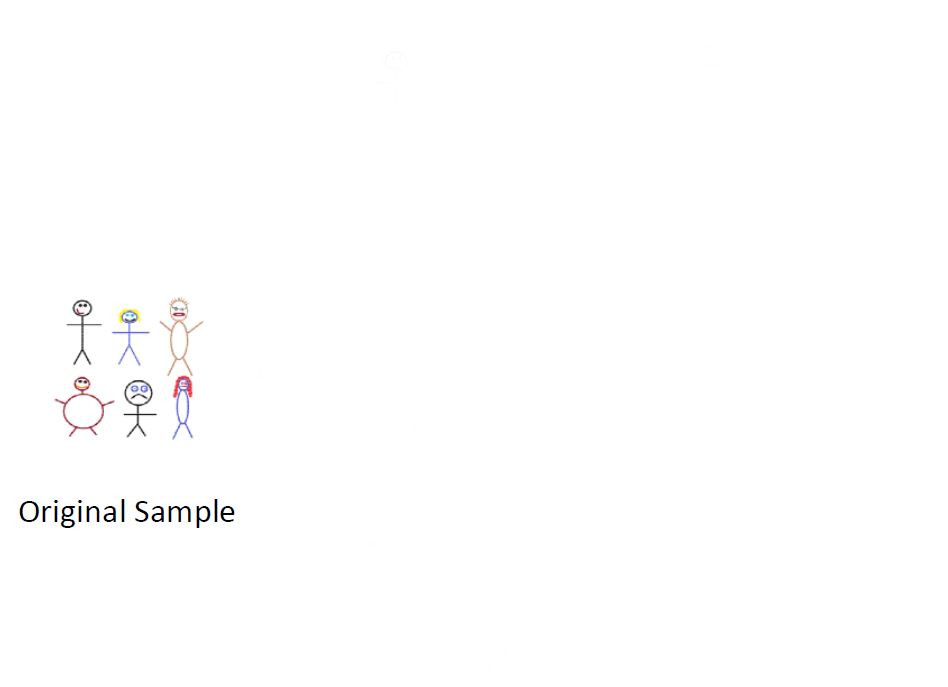
\includegraphics[width=.75\textwidth]{sample1.JPG}}
\only<3>{\textbf{What is the CI for the average height?}}
\only<4>{\hspace{-.055in}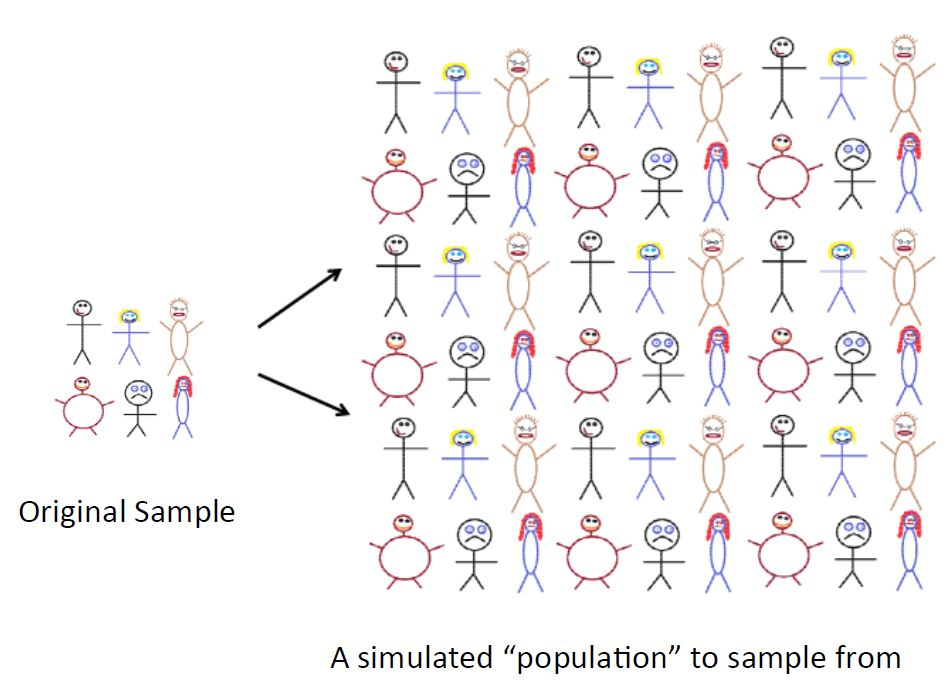
\includegraphics[width=.75\textwidth]{sample2.JPG}}
\only<5>{\hspace{-.1in}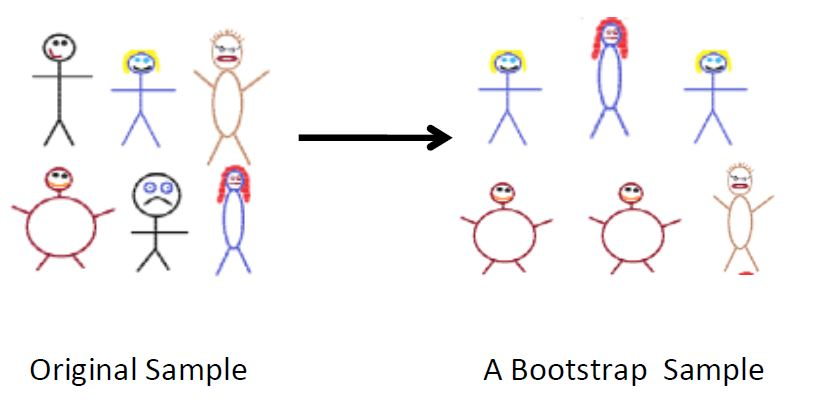
\includegraphics[width=.75\textwidth]{sample3.JPG}}
\only<6>{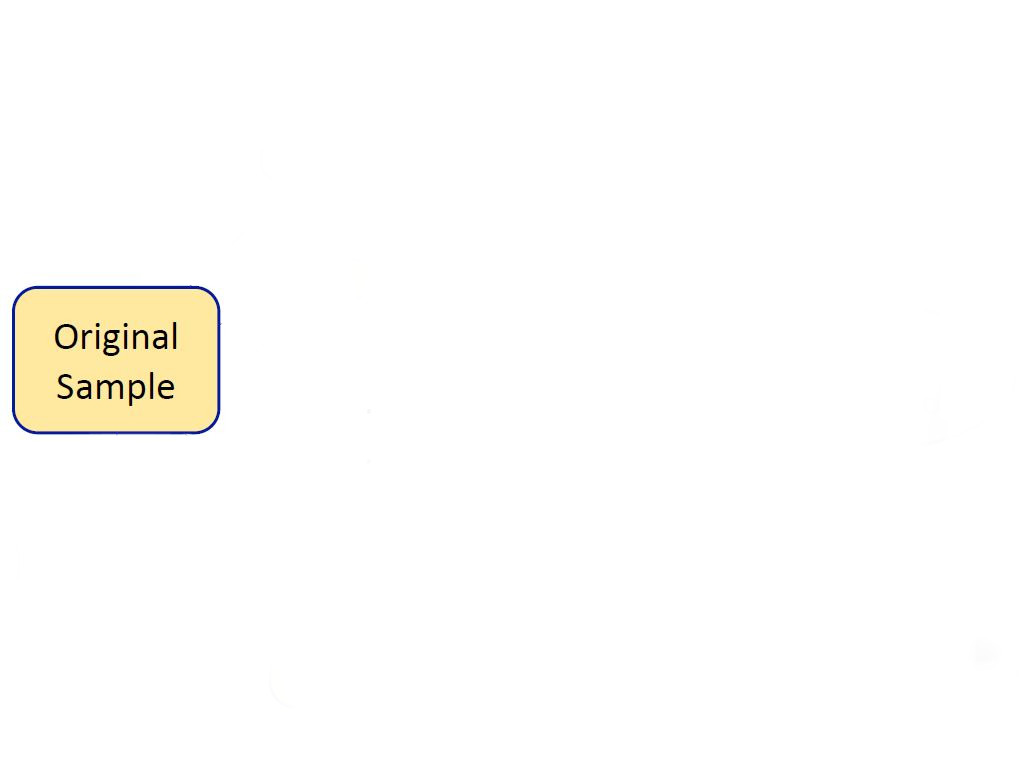
\includegraphics[width=.75\textwidth]{flowchart1.JPG}}
\only<7>{\hspace{-.05in}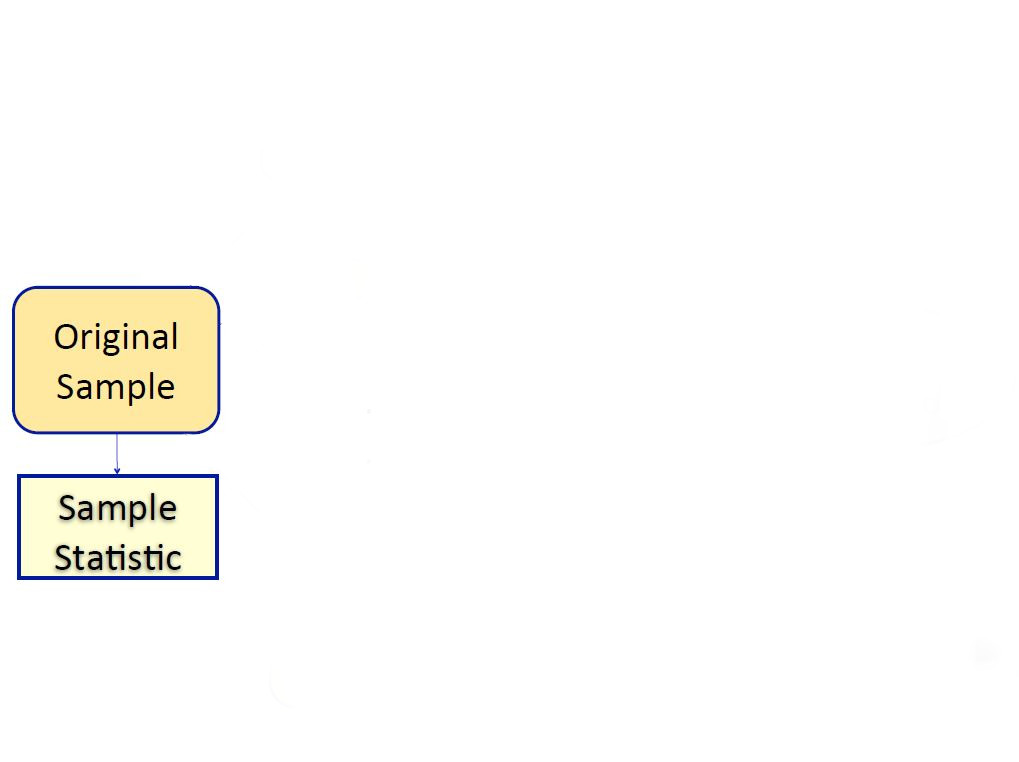
\includegraphics[width=.75\textwidth]{flowchart2.JPG}}
\only<8>{\hspace{-.105in}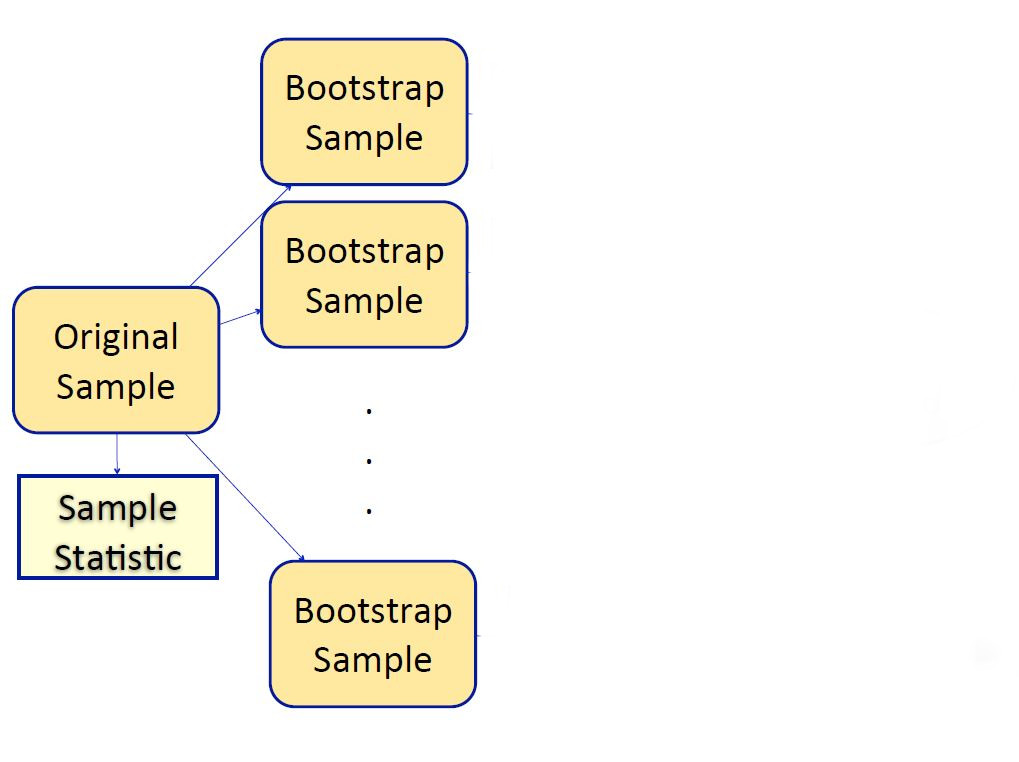
\includegraphics[width=.75\textwidth]{flowchart3.JPG}}
\only<9>{\hspace{-.16in}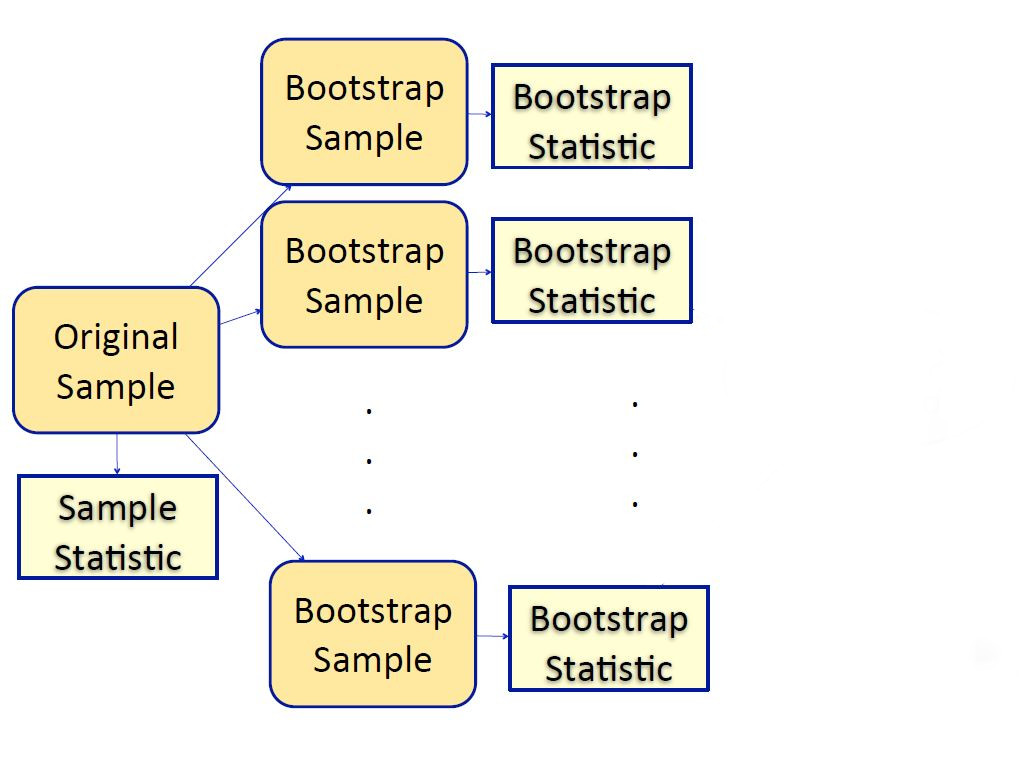
\includegraphics[width=.75\textwidth]{flowchart4.JPG}}
\only<10>{\hspace{-.215in}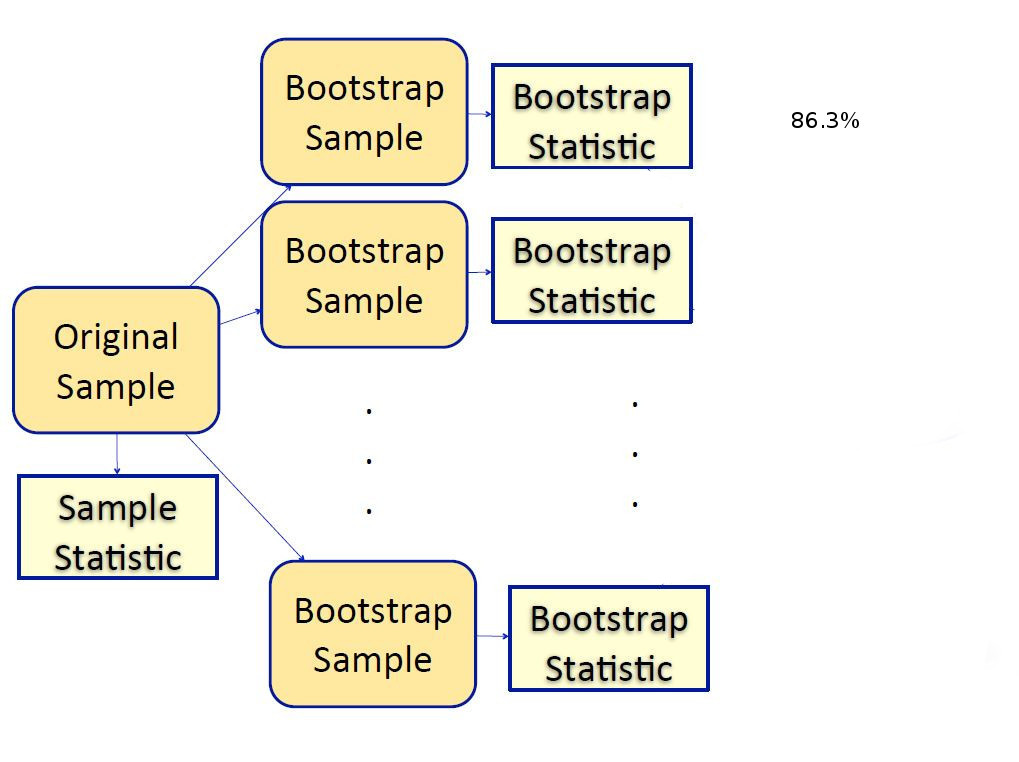
\includegraphics[width=.75\textwidth]{flowchart5.JPG}}
\only<11>{\hspace{-.27in}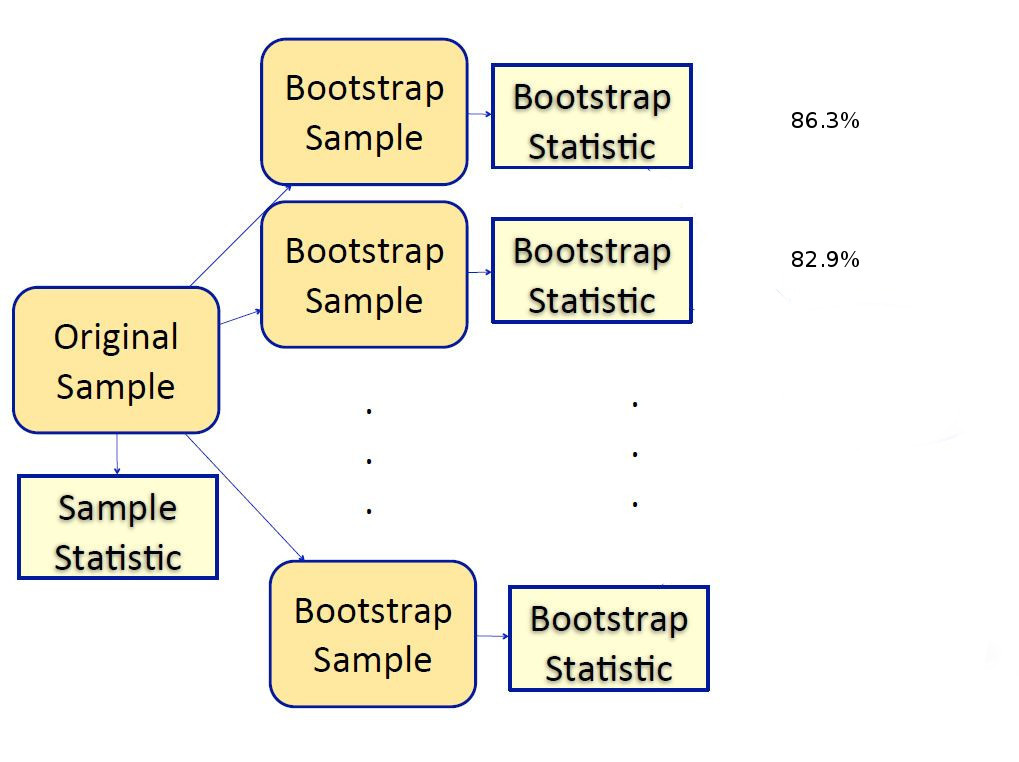
\includegraphics[width=.75\textwidth]{flowchart6.JPG}}
\only<12>{\hspace{-.325in}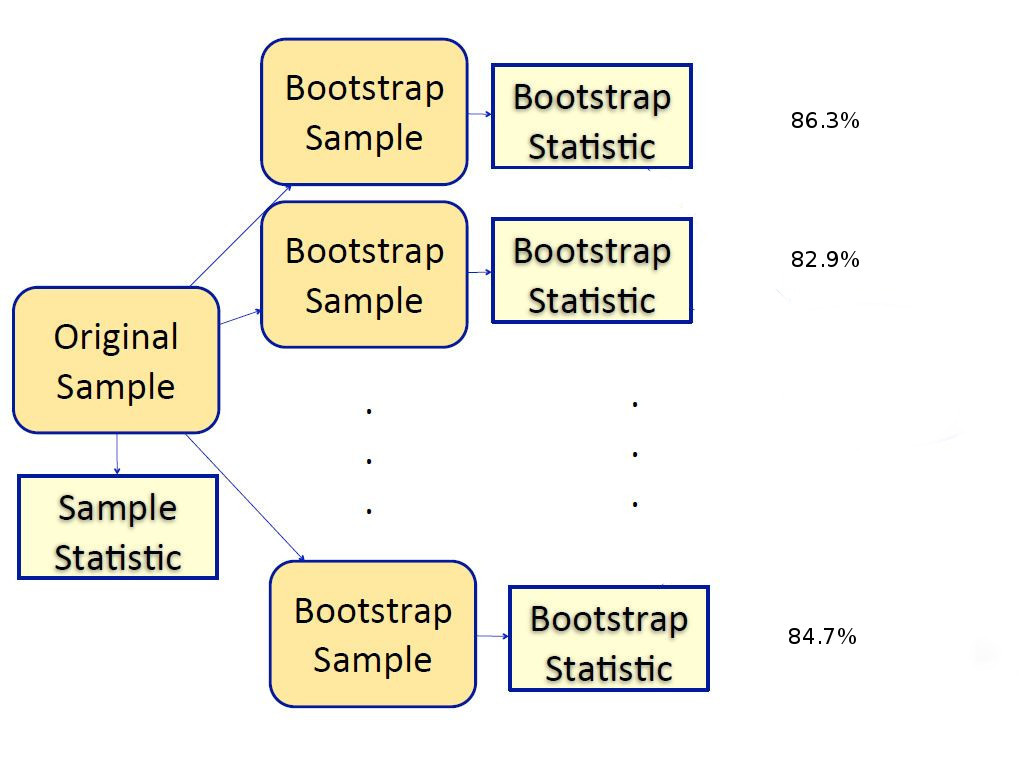
\includegraphics[width=.75\textwidth]{flowchart7.JPG}}
\only<13>{\hspace{-.38in}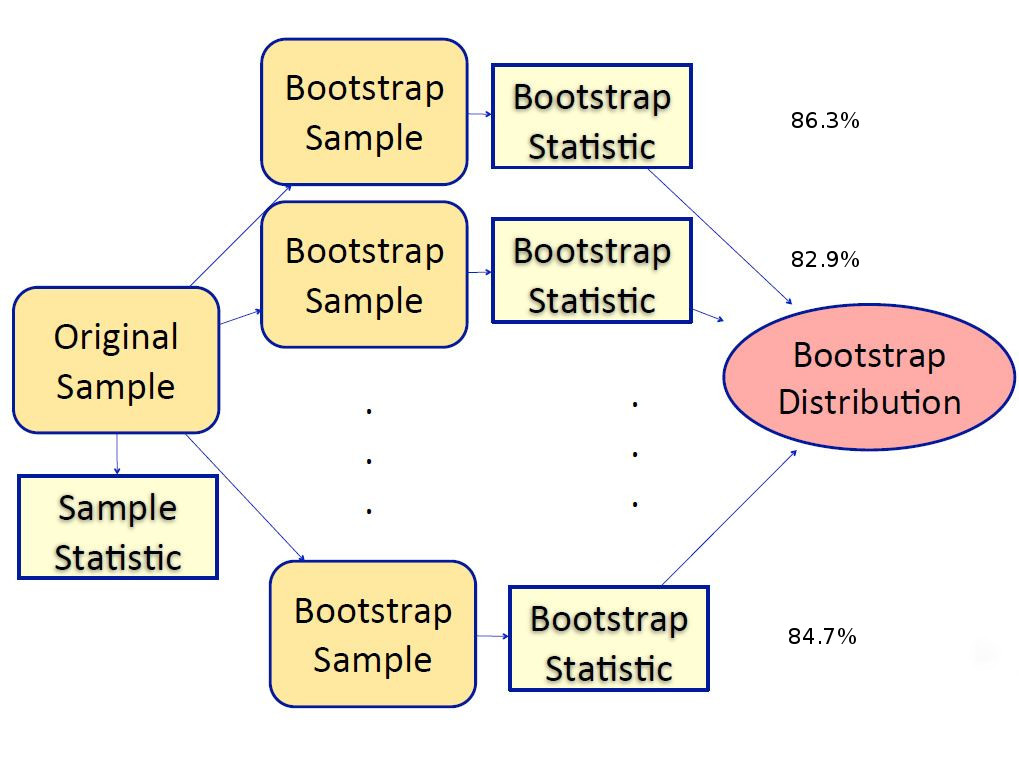
\includegraphics[width=.75\textwidth]{flowchart8.JPG}}
\only<14>{\hspace{-.435in}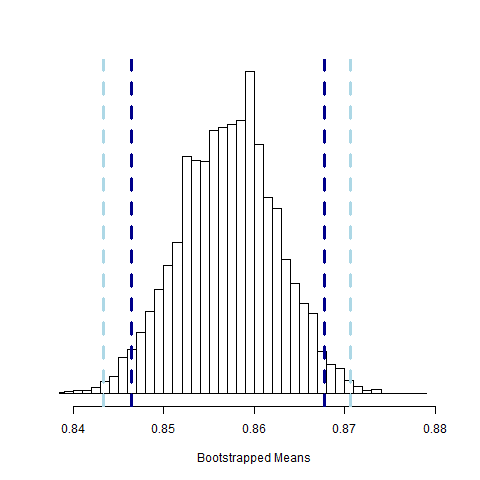
\includegraphics[width=.55\textwidth]{bootdist1.JPG}}



\end{frame}
}


\begin{frame}[fragile]
\ttfamily
\frametitle{R Coding: The American National Election Study}

\only<2-5>{
\uncover<2->{
X = mean(anes16\$registered)\\
X   \# 0.857\\
}
\vspace{.1in}
\uncover<3->{
SD = sd(anes16\$registered)\\
SD   \# 0.350\\
}
\vspace{.1in}
\uncover<4->{
SE = SD/sqrt(nrow(anes16))\\
SE   \# 0.005\\
}
\vspace{.1in}
\uncover<5->{
X + 1.96*SE   \# 0.868\\
X - 1.96*SE   \# 0.848\\
}}

\only<6-14>{

\uncover<11->{
\textcolor{blue}{bootstrapped.distribution = \spot<11>{replicate}(\spot<12>{100}, \texttt{\{}
}}\\
\uncover<6->{
\hspace{.2in} bootstrapped.sample = \spot<7>{mosaic::shuffle}(\spot<8>{anes16}, \spot<9>{replace=TRUE})
}\\
\uncover<6->{
\hspace{.2in} \spot<10>{mean}(bootstrapped\$registered) \\
}
\uncover<11->{
\textcolor{blue}{\texttt{\}})}\\
}
\uncover<13->{
\textcolor{junglegreen}{
quants = \spot<13>{quantile}(bootstrapped.distribution, c(0.025, 0.975))\\
quants} \# 0.846, 0.867
}

\vspace{.3in}

\uncover<14->{
\textsf{\textbf{How many bootstrapped samples do we generate?}}
}
}

\only<15>{
\centering
\hspace{.525in}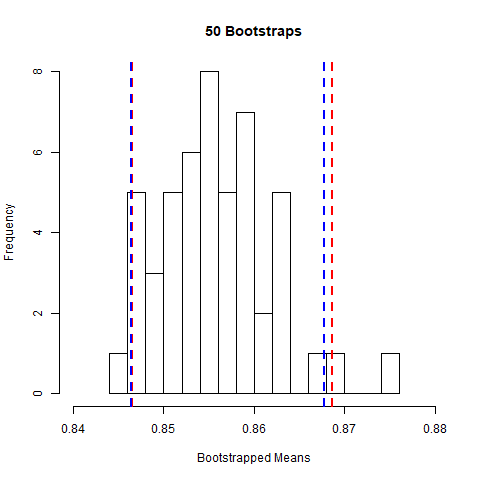
\includegraphics[width=0.55\textwidth]{hist1.jpg}
}
\only<16>{
\centering
\hspace{.45in}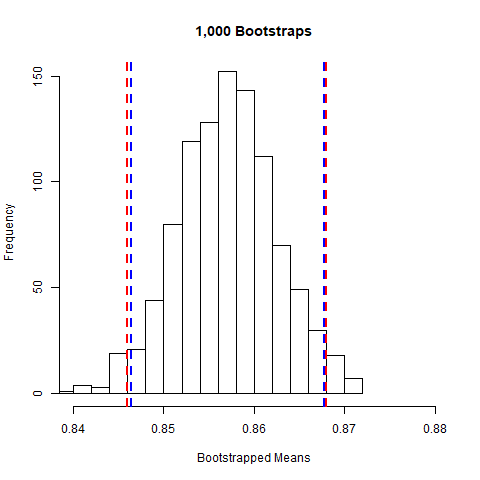
\includegraphics[width=0.55\textwidth]{hist2.jpg}
}
\only<17>{
\centering
\hspace{.35in}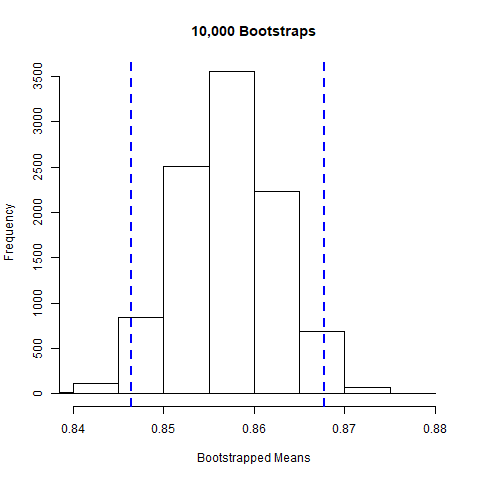
\includegraphics[width=0.55\textwidth]{hist3.jpg}
}

\only<18>{
\textsf{But we can also bootstrap more complicated stuff!}\\
\vspace{.2in}
\textcolor{junglegreen}{cor(anes16\$age, anes16\$registered)} \# 0.199 
}



\only<19-24>{

\uncover<23->{
\textcolor{blue}{bootstrapped.corr = replicate(100, \texttt{\{}
}}\\
\uncover<19->{
\hspace{.2in} bootstrapped.sample = mosaic::shuffle(anes16,replace=TRUE)
}\\
\uncover<20->{
\hspace{.2in} \spot<21>{cor}(bootstrapped.sample\$registered, \spot<22>{bootstrapped.sample\$age}) \\
}
\uncover<23->{
\textcolor{blue}{\texttt{\}})}\\
}
\uncover<24->{
\textcolor{junglegreen}{
corrs = \spot<24>{quantile}(bootstrapped.corr, c(0.025, 0.975))\\
corrs} \# 0.173, 0.230
}
}
\end{frame}



\begin{frame}
\frametitle{Even more complicated stuff}
\only<1>{
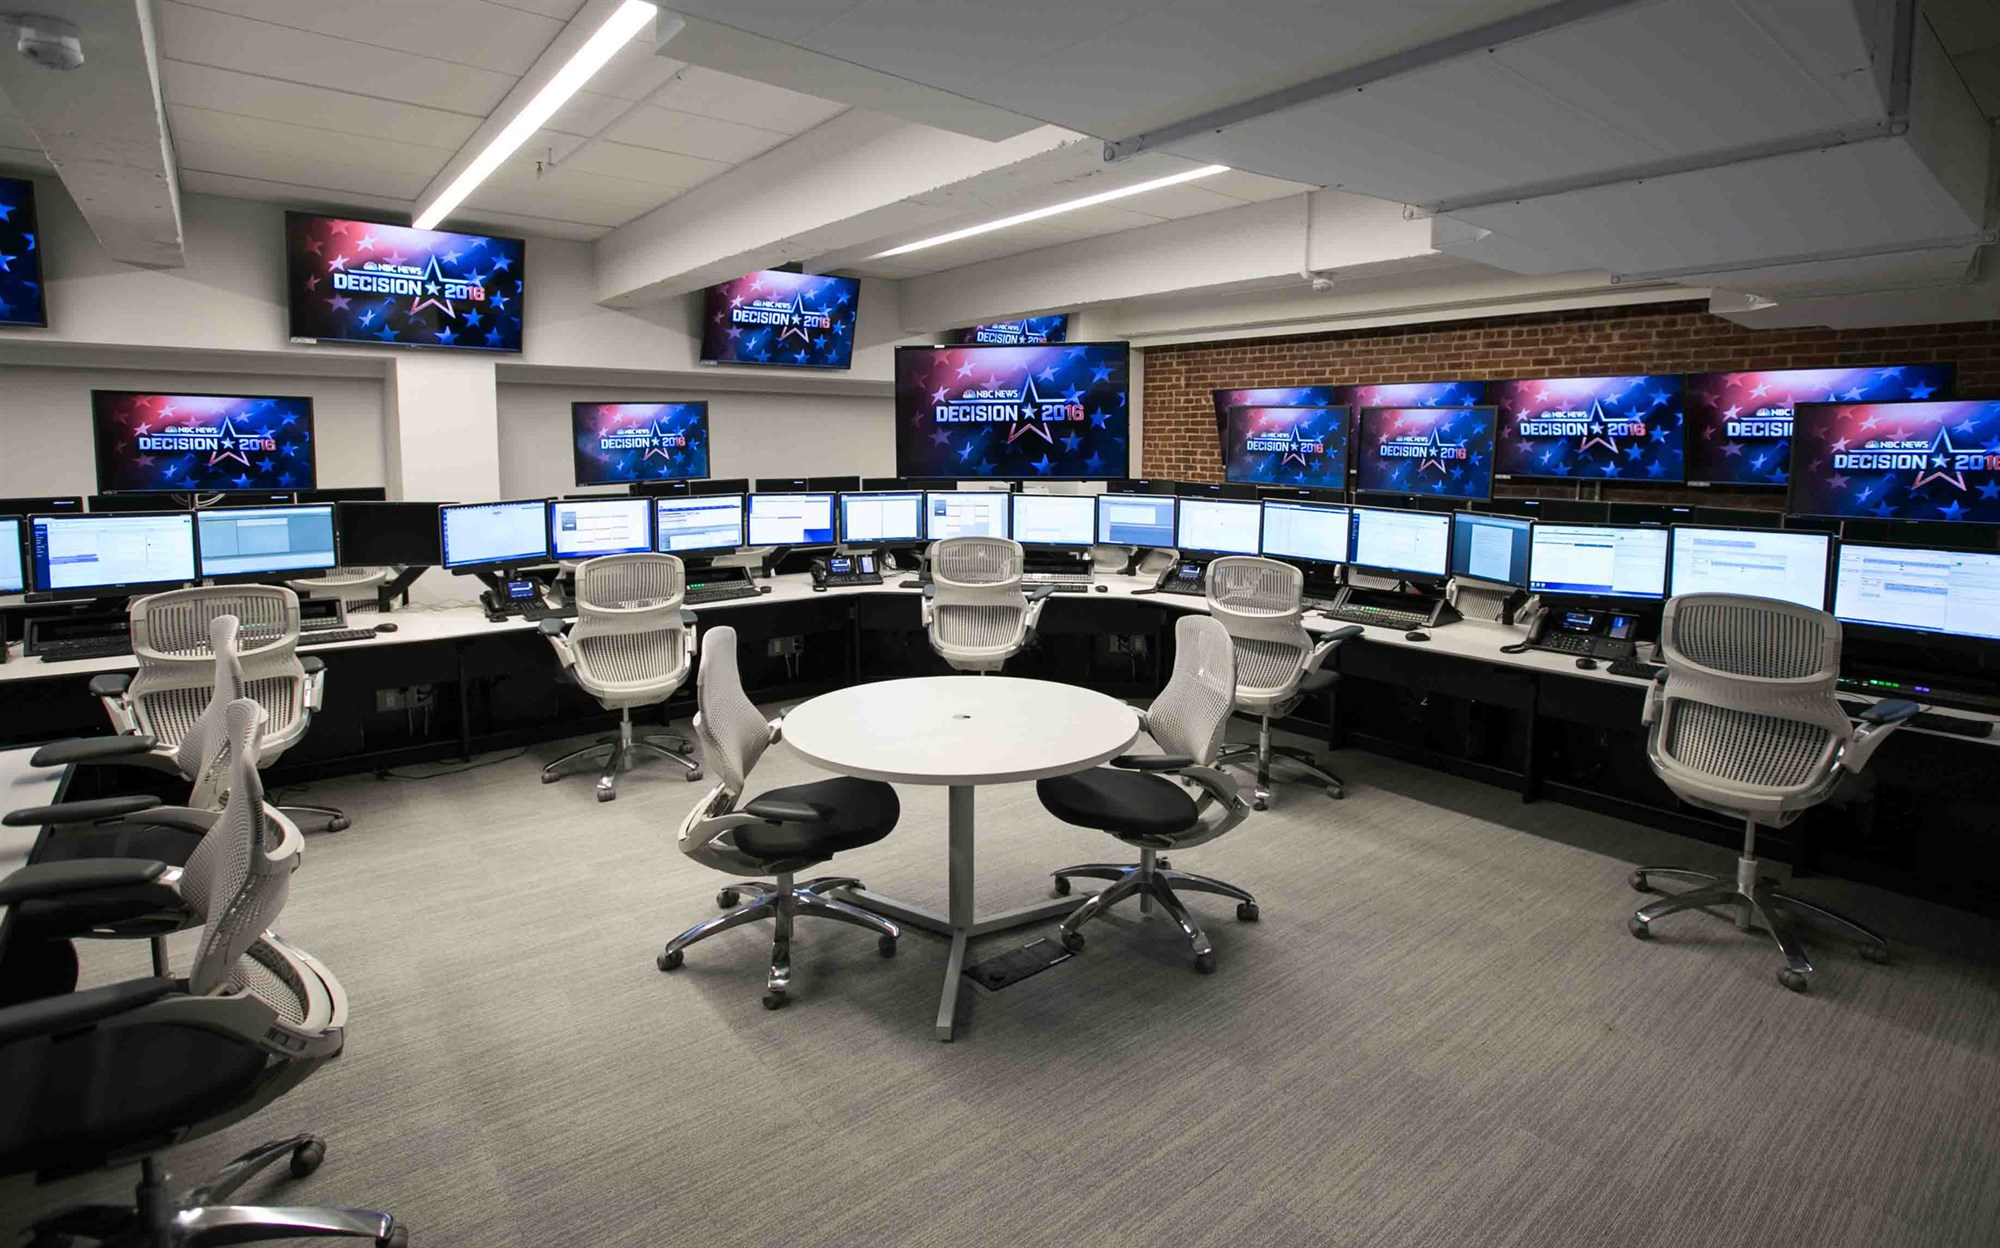
\includegraphics[width = .9\textwidth]{decisiondesk.jpg}
}

\only<2-5>{

\textbf{How do they ``call'' an election?} How do they call elections with only 1\% of the data?

\begin{itemize}
\item<3->{Build a model to predict the election}
\item<4->{How do calculate uncertainty?}
\item<5->{\textbf{Bootstrap!}}
\end{itemize}

}


\only<6-20>{

\textbf{When can we ``call'' an election?}  \uncover<7->{When 99\% CI only contains one winner} 

\vspace{.1in}
\uncover<8->{
\textcolor{blue}{bootstrapped.corr = replicate(100, \texttt{\{}
}}\\
\uncover<9->{
\hspace{.2in} bootstrapped.sample = mosaic::shuffle(\spot<10>{election.returns},replace=TRUE)
}\\
\uncover<11->{
\hspace{.2in} model = \spot<12>{lm}(\spot<13>{DemWins18} $\sim$ \spot<14>{VoteSoFar} + \spot<15>{DemPct16} + pctWhite, \\ 
\hspace{.4in} bootstrapped.sample)
}\\
\uncover<16->{
\hspace{.2in} preds = \spot<17>{predict}(m, newdata = data.frame(\spot<18>{VoteSoFar = 0.65}, \\
\hspace{.4in} \spot<19>{DemPct16 = 0.75}, \spot<20>{pctWhite = 0.4}) 
}\\
\uncover<8->{
\textcolor{blue}{\texttt{\}})}\\
}
}



\end{frame}




%% Summary slide:
% 1) The bootstrap is a computational approach when analytic approaches fail (or we just don't want to use them)
% 2) It involves resampling our full data set WITH REPLACEMENT, then calculating our QOI
% 3) It makes it easier to calculate confidence intervals of different confidences (90, 95, 99.9999, etc)
% 4) It works for complicated stuff too! [Example from my work]

% Some coding tips when doing this:
% 1) The mosaic R package includes the shuffle() function: shuffle(dat, replace=FALSE)
% 2) The replicate() function repeats a snippet of code however many times you want
% 3) calculate quantiles: quantile(bootstrapped.avgs, c(0.025, 0.975))


\begin{frame}
\frametitle{Summary \& Coding tips}

\uncover<2->{\textbf{The bootstrap...}}
\begin{enumerate}
	\item<3->{Involves resampling the full data \alert{with replacement}}
	\item<4->{Is useful when analytic approaches fail (or when we are feeling lazy)}
	\item<5->{Works for complicated sample statistics too: \uncover<6->{correlations,}\uncover<7->{ predictions,}\uncover<8->{ modeling accuracy...}} 
\end{enumerate}

\uncover<9->{\textbf{To make it easier...}}
\begin{itemize}
	\item<10->{Use the \texttt{replicate()} function to repeat your resampling lots of times}
	\item<11->{Use the \texttt{shuffle()} function from the \texttt{mosaic} library: \uncover<12->{\texttt{mosaic::shuffle(dat, replace=FALSE)}}}
	\item<13->{Calculate quantiles: \uncover<14->{\texttt{quantile(bootstrapped.avgs, c(0.025, 0.975))}}}
\end{itemize}
\end{frame}

%% Wrap up frame with a link to the code here

\begin{frame}
\frametitle{Thank you!}

\textbf{\LaTeX, R code, and data at:} \\
\vspace{.2in}
\url{http://www.github.com/aaronrkaufman/bootstrap}


\end{frame}


\end{document}


%%% Talk about how it fails over the support